\documentclass{article}
% Change "article" to "report" to get rid of page number on title page
\usepackage{amsmath,amsfonts,amsthm,amssymb}
\usepackage{setspace}
\usepackage{Tabbing}
\usepackage{fancyhdr}
\usepackage{lastpage}
\usepackage{extramarks}
\usepackage{chngpage}
\usepackage{soul,color}
\usepackage{graphicx,float,wrapfig}
\usepackage{multirow}
\usepackage{enumerate}
% In case you need to adjust margins:
\topmargin=-0.45in      %
\evensidemargin=0in     %
\oddsidemargin=0in      %
\textwidth=6.5in        %
\textheight=9.0in       %
\headsep=0.25in         %

% Homework Specific Information
\newcommand{\hmwkTitle}{Mini-Report:Decompose Restaurant}
\newcommand{\hmwkClass}{}
\newcommand{\hmwkAuthorName}{Donglai\ Wei}


% Setup the header and footer
\pagestyle{fancy}                                                       %
\lhead{\hmwkAuthorName}                                                 %
\rhead{\firstxmark}                                                     %
\lfoot{\lastxmark}                                                      %
\cfoot{}                                                                %
\rfoot{Page\ \thepage\ of\ \pageref{LastPage}}                          %
\renewcommand\headrulewidth{0.4pt}                                      %
\renewcommand\footrulewidth{0.4pt}                                      %

% This is used to trace down (pin point) problems
% in latexing a document:
%\tracingall

%%%%%%%%%%%%%%%%%%%%%%%%%%%%%%%%%%%%%%%%%%%%%%%%%%%%%%%%\begin{enumerate}

% Some tools
\newcommand{\enterProblemHeader}[1]{\nobreak\extramarks{#1}{#1 continued on next page\ldots}\nobreak%
                                    \nobreak\extramarks{#1 (continued)}{#1 continued on next page\ldots}\nobreak}%
\newcommand{\exitProblemHeader}[1]{\nobreak\extramarks{#1 (continued)}{#1 continued on next page\ldots}\nobreak%
                                   \nobreak\extramarks{#1}{}\nobreak}%

\newlength{\labelLength}
\newcommand{\labelAnswer}[2]
  {\settowidth{\labelLength}{#1}%
   \addtolength{\labelLength}{0.25in}%
   \changetext{}{-\labelLength}{}{}{}%
   \noindent\fbox{\begin{minipage}[c]{\columnwidth}#2\end{minipage}}%
   \marginpar{\fbox{#1}}%

   % We put the blank space above in order to make sure this
   % \marginpar gets correctly placed.
   \changetext{}{+\labelLength}{}{}{}}%

\setcounter{secnumdepth}{0}
\newcommand{\homeworkProblemName}{}%
\newcounter{homeworkProblemCounter}%
\newenvironment{homeworkProblem}[1][Problem \arabic{homeworkProblemCounter}]%
  {\stepcounter{homeworkProblemCounter}%
   \renewcommand{\homeworkProblemName}{#1}%
   \section{\homeworkProblemName}%
   \enterProblemHeader{\homeworkProblemName}}%
  {\exitProblemHeader{\homeworkProblemName}}%

\newcommand{\problemAnswer}[1]
  {\noindent\fbox{\begin{minipage}[c]{\columnwidth}#1\end{minipage}}}%

\newcommand{\problemLAnswer}[1]
  {\labelAnswer{\homeworkProblemName}{#1}}

\newcommand{\homeworkSectionName}{}%
\newlength{\homeworkSectionLabelLength}{}%
\newenvironment{homeworkSection}[1]%
  {% We put this space here to make sure we're not connected to the above.
   % Otherwise the changetext can do funny things to the other margin

   \renewcommand{\homeworkSectionName}{#1}%
   \settowidth{\homeworkSectionLabelLength}{\homeworkSectionName}%
   \addtolength{\homeworkSectionLabelLength}{0.25in}%
   \changetext{}{-\homeworkSectionLabelLength}{}{}{}%
   \subsection{\homeworkSectionName}%
   \enterProblemHeader{\homeworkProblemName\ [\homeworkSectionName]}}%
  {\enterProblemHeader{\homeworkProblemName}%

   % We put the blank space above in order to make sure this margin
   % change doesn't happen too soon (else \sectionAnswer's can
   % get ugly about their \marginpar placement.
   \changetext{}{+\homeworkSectionLabelLength}{}{}{}}%

\newcommand{\sectionAnswer}[1]
  {% We put this space here to make sure we're disconnected from the previous
   % passage

   \noindent\fbox{\begin{minipage}[c]{\columnwidth}#1\end{minipage}}%
   \enterProblemHeader{\homeworkProblemName}\exitProblemHeader{\homeworkProblemName}%
   \marginpar{\fbox{\homeworkSectionName}}%

   % We put the blank space above in order to make sure this
   % \marginpar gets correctly placed.
   }%

%%%%%%%%%%%%%%%%%%%%%%%%%%%%%%%%%%%%%%%%%%%%%%%%%%%%%%%%%%%%%



%%%%%%%%%%%%%%%%%%%%%%%%%%%%%%%%%%%%%%%%%%%%%%%%%%%%%%%%%%%%%
% Make title
\title{\vspace{0.3in}\textmd{\textbf{\hmwkTitle}}}
\date{2010.6.16}
\author{\textbf{\hmwkAuthorName}}
%%%%%%%%%%%%%%%%%%%%%%%%%%%%%%%%%%%%%%%%%%%%%%%%%%%%%%%%%%%%%

\begin{document}
\begin{spacing}{1.1}
\maketitle


\section{1) Algorithm}
GOAL: Maximize log Probability P=$log p(x,z|\lambda,\alpha,\gamma)$
\begin{enumerate}[(i)]
\item Make Restaurant j into one table t1 where customers following uniform distribution
\item Iterate until no customers are left in this uniform table t1:
\begin{enumerate}
\item For each dish k, propose to form a new table$^{1*}$ out of t1 with dish k and calculate the weight $\Delta P$
\item Sample$^{2*}$ a proposal according to the weight and make the new table
\end{enumerate}
\item TKM$^{3*}$
\item Decision$^{4*}$
\end{enumerate}
{\bf NOTE:}:\\
$^{1*}$:One naive proposal is to assign customers with overlapped words between t1 and dish k to the new table. But actually, it is a only rough 
approximation of the "best" new table can be made by dish k: threshold $\frac{n_{..k}^{w}+\phi_{0}}{{n_{..k}+W\phi_{0}}}\sim\frac{n_{..k}^{w}}{n_{..k}}$ of the overlapped word w by $\frac{1}{W}$\\ \\
$^{2*}$:$\Delta P$ has nothing to do with Probability and different scalings lead to different functionality(variability or peaky)\\ \\
$^{3*}$:In practice, merge table may not be a good idea since it's a little too greedy while the dishes are still fledging. In Local Search k,
we can also restrict the tables not to have new dishes, forcing Restaurant j to be explained by old dishes.\\ \\
$^{4*}$ Accept all or Reject if decrease P

\section{2) Experiment}
\subsection{i)  Empirical Results}
$^{0*}$:In general, Decompose Restaurant can roughly find the bars from the darkness.(See Figure 2 right)\\ \\
$^{1*}$:Proposal with threshold works better. Simply we don't want to accumulate the noise in the dish .\\ \\
$^{2*}$:During Initialization, greedy assignment is better than sampling.\\ \\
$^{3*}$:Allowing new dishes in local search k works a little better.\\ \\
$^{4*}$:During Initialization, we'd better accept all new configurations which may decrease P by splitting up noisy tables.\\ \\
\subsection{ii) Problems{\small (left for Decompose Dish)}}
1) Decompose Restaurant(DR) cannot further purify the dishes.\\ \\
Since the algorithm only considers one new table at a time(a little greedy), it fails to favor pairs of dishes over one bigger dish.\\
Thus, if a mixture of bars happen several times, Decompose Restaurant may make it a dish even though the bars have been figured out elsewhere.\\ \\
In Figure 1 are one restaurant and three dishes. Though the words in dish right has smaller 
words frequency, it rescues more of the uniform distributed words. Thus the Restaurant may not want to be explained by the other two dishes, even we do sampling. 
\begin{figure}
 \centering
    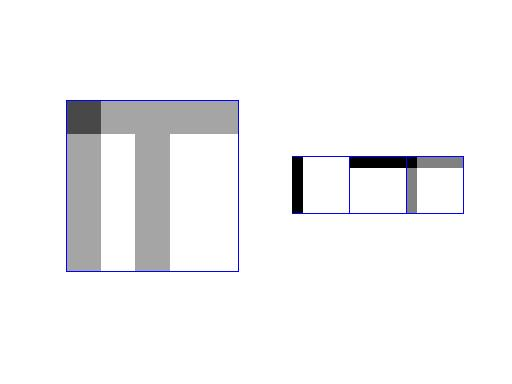
\includegraphics[width=2.5in,height=2in]{eg.jpg} 
    \caption{DR may favor mixture of bars(right) instead of pure bars(left,middle)}
    \label{fig:by:table} 
\end{figure}

\newpage
\subsection{iii)200 5*5 matrix}

\begin{figure}
 \centering
   \begin{tabular}{cc}    
     \resizebox{50mm}{!}{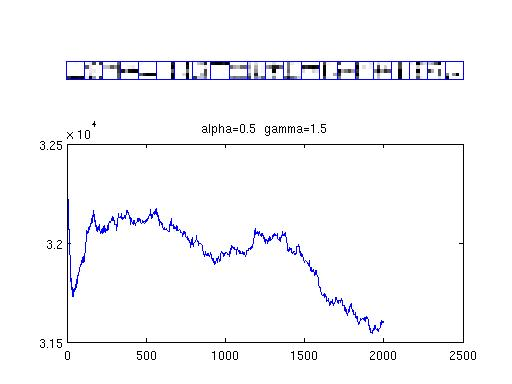
\includegraphics{a_ns_new.jpg}} &
     \resizebox{50mm}{!}{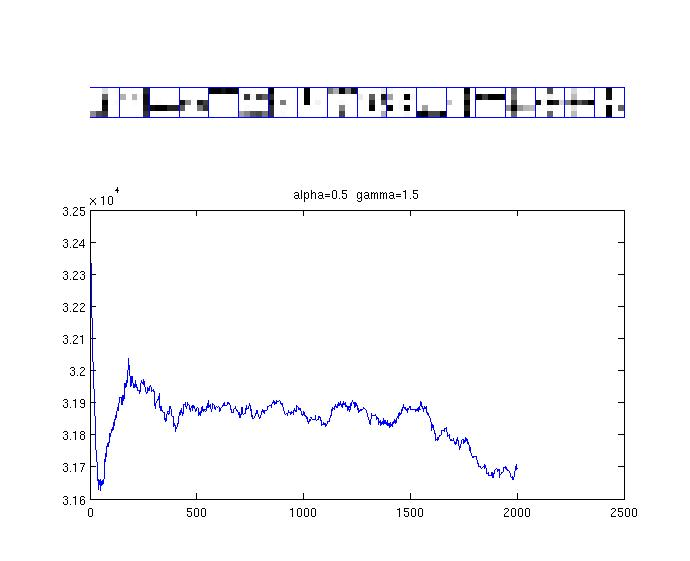
\includegraphics{a_ns_new_nover.jpg}} \\
   \end{tabular}
    \caption{1)Proprosal to make new table with threshold(right) works better}
    \label{fig:by:table} 
\end{figure}

\begin{figure}
  \begin{center}
    \begin{tabular}{cc}
      \resizebox{50mm}{!}{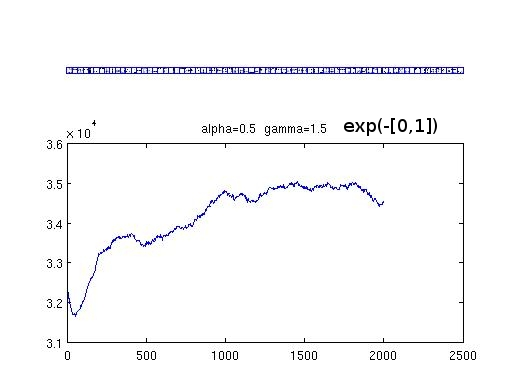
\includegraphics{a_s1_nonew.jpg}} &
      \resizebox{50mm}{!}{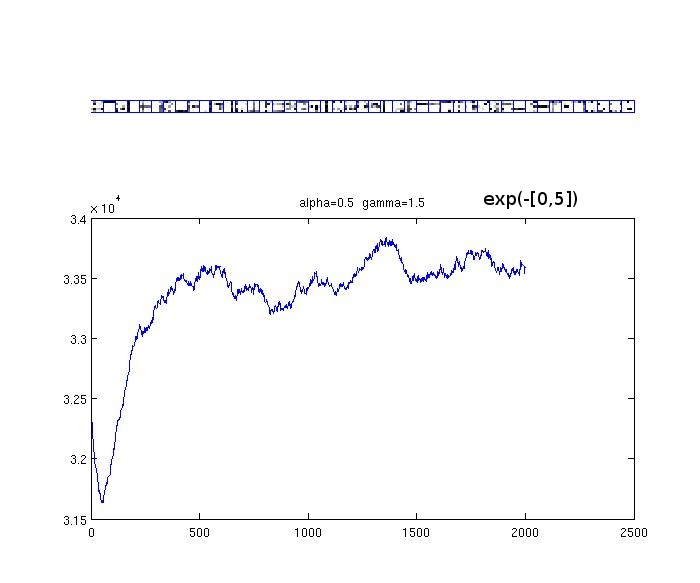
\includegraphics{a_s5_nonew.jpg}} \\
      \resizebox{50mm}{!}{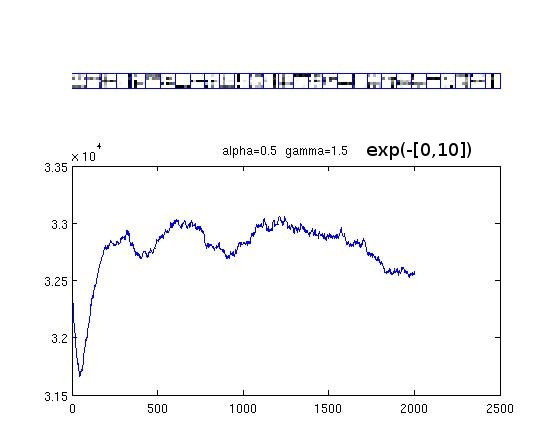
\includegraphics{a_s10_nonew.jpg}} &
      \resizebox{50mm}{!}{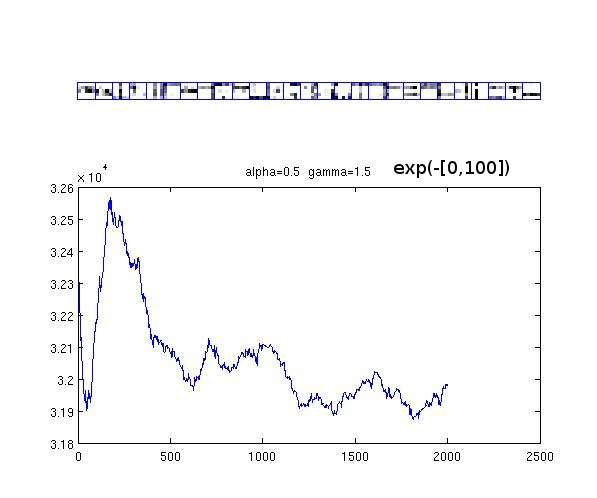
\includegraphics{a_s100_nonew.jpg}} \\
    \end{tabular}
    \caption{2)Scale the weight to [0,r],then sample from exp(-weight),peeky works better(down-right)}
     \label{fig:by:table} 
  \end{center}
\end{figure}
\begin{figure}
 \centering
   \begin{tabular}{cc}    
     \resizebox{60mm}{!}{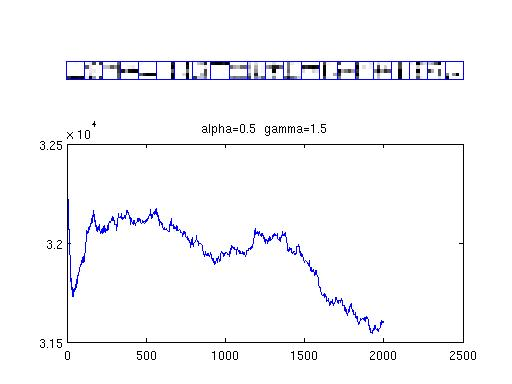
\includegraphics{a_ns_new.jpg}} &
     \resizebox{60mm}{!}{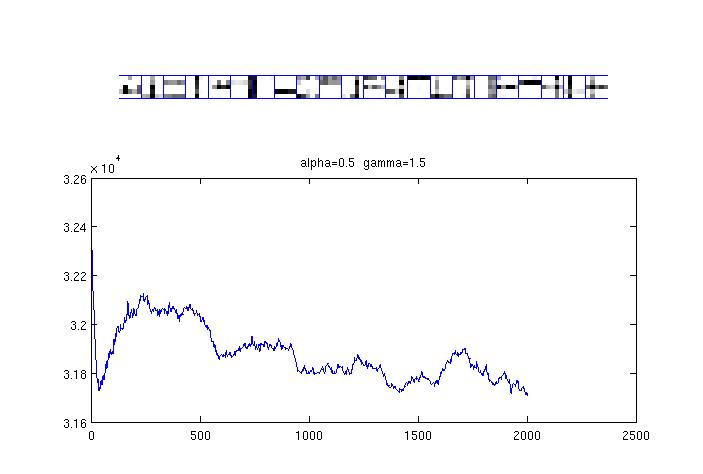
\includegraphics{a_ns_nonew.jpg}} \\
   \end{tabular}
    \caption{3)Local Search K: allowing new dishes(left) works better than the opposite(right)}
    \label{fig:by:table} 
\end{figure}

\begin{figure}
 \centering
   \begin{tabular}{cc}    
     \resizebox{60mm}{!}{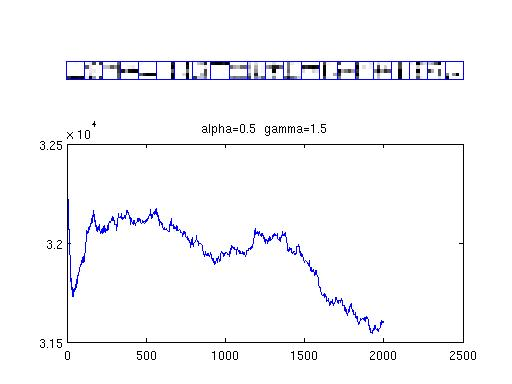
\includegraphics{a_ns_new.jpg}} &
     \resizebox{60mm}{!}{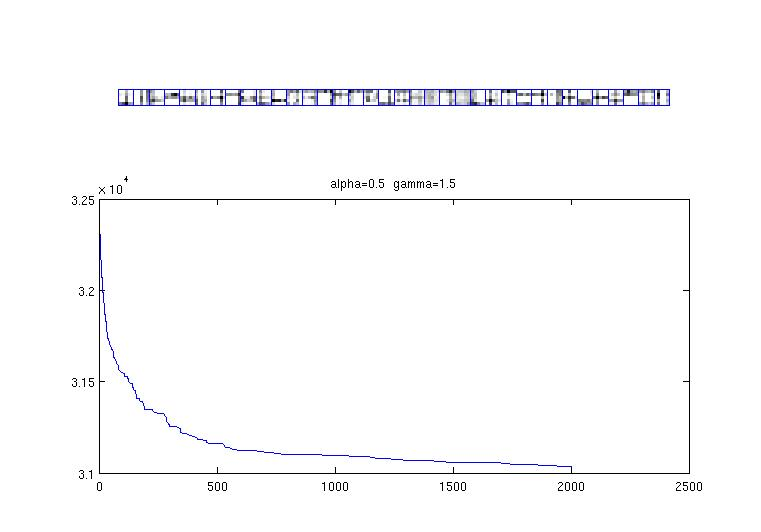
\includegraphics{r_ns_new.jpg}} \\
   \end{tabular}
    \caption{4)Accept all configurations(left) works better than Accept/Reject(right)}
    \label{fig:by:table} 
\end{figure}

\end{spacing}
\end{document}

%%%%%%%%%%%%%%%%%%%%%%%%%%%%%%%%%%%%%%%%%%%%%%%%%%%%%%%%%%%%%
